\documentclass[aspectratio=169,11pt]{beamer}
 
\usepackage[utf8]{inputenc}
\usepackage[T1]{fontenc}
\usepackage[slovene]{babel}
\usepackage{graphicx}
\usepackage{booktabs}
\usepackage{amsmath}
 
\usetheme{Madrid}
\usecolortheme{default}
\setbeamertemplate{navigation symbols}{}
 
\title[Zaznavanje in razmejevanje posameznih borovnic]{Zaznavanje in razmejevanje posameznih borovnic na slikah}
\subtitle{Kratka Predstavitev}
\author{Lan Stare}
\institute[FMF]{Fakulteta za matematiko in fiziko, Univerza v Ljubljani}
\date{\today}
 
\begin{document}
 
% 1. Naslov
\begin{frame}
  \titlepage
  \vfill
  {\small Mentor: prof. dr. Ljupčo Todorovski \quad Somentor: znan. sod. dr. Domen Tabernik}
\end{frame}
 
% 2. Razlaga teme
\begin{frame}{Področje}
    \begin{block}{Definicija}
      \textbf{Umetna inteligenca (AI):} Področje računalništva, ki se ukvarja z razvojem sistemov, sposobnih opravljati naloge, za katere je običajno potrebna človeška inteligenca.
    \end{block}
    \begin{block}{Definicija}
      \textbf{Strojno učenje:} Področje umetne inteligence, ki razvija algoritme in modele, ki se učijo vzorcev iz podatkov ter na njihovi podlagi sprejemajo odločitve ali napovedujejo rezultate.
    \end{block}
    \begin{block}{Definicija}
      \textbf{Nevronske mreže:} Modeli strojnega učenja, sestavljeni iz medsebojno povezanih nevronov, ki z učenjem iz podatkov lahko prepoznavajo kompleksne vzorce.\\
      \textbf{Konvolucijske nevronske mreže:} Vrsta nevronskih mrež, ki samodejno prepoznavajo prostorske značilnosti podatkov, še posebej na slikah in videoposnetkih.
    \end{block}
\end{frame}

\begin{frame}{Razlaga teme}
  \begin{columns}[T]
    \column{0.55\textwidth}
    \begin{itemize}
      \item \textbf{Zaznavanje (detection)}: Prepoznavanje in določanje položaja objektov na slikah ali videoposnetkov (določanje položaja vsake borovnice na sliki)
      \item \textbf{Razmejevanje (segmentation)}: Razvrstitev vsake pike na sliki v svojo kategorijo za natančno določitev oblike predmetov
      \item \textbf{Razmejevanje posameznih objektov (instance segmentation)}: določanje območja in oblike vsakega posameznega objekta na sliki z razvrščanjem slikovnih pik glede na pripadnost posameznemu objektu in njegovi kategoriji (zrela, polzrela ali nezrela borovnica oz. ozadje)
    \end{itemize}
    \column{0.4\textwidth}
    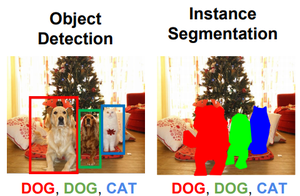
\includegraphics[width=\textwidth]{slike/detection_segmentation.png}
    \par\smallskip
    \centering{\scriptsize Vir: \href{https://www.geeksforgeeks.org/machine-learning/object-detection-vs-object-recognition-vs-image-segmentation/}{GeeksforGeeks}}
  \end{columns}
\end{frame}

% 3. Motivacija in problem
\begin{frame}{Motivacija in problem}
  \begin{columns}[T]
    \column{0.55\textwidth}
    \begin{itemize}
       
      \item Zakaj zrelost borovnic?\\Zaradi manjšanja števila kmetov koristi avtomatizirano obiranje z robotom
      \item Problemi:
        \begin{itemize}
          \item majhni plodovi
          \item prekrivanje
          \item majhna razlika v barvi
          \item zamegljenost
          \item neenakomerna porazdelitev razredov
        \end{itemize}
    \end{itemize}
    \column{0.4\textwidth}
    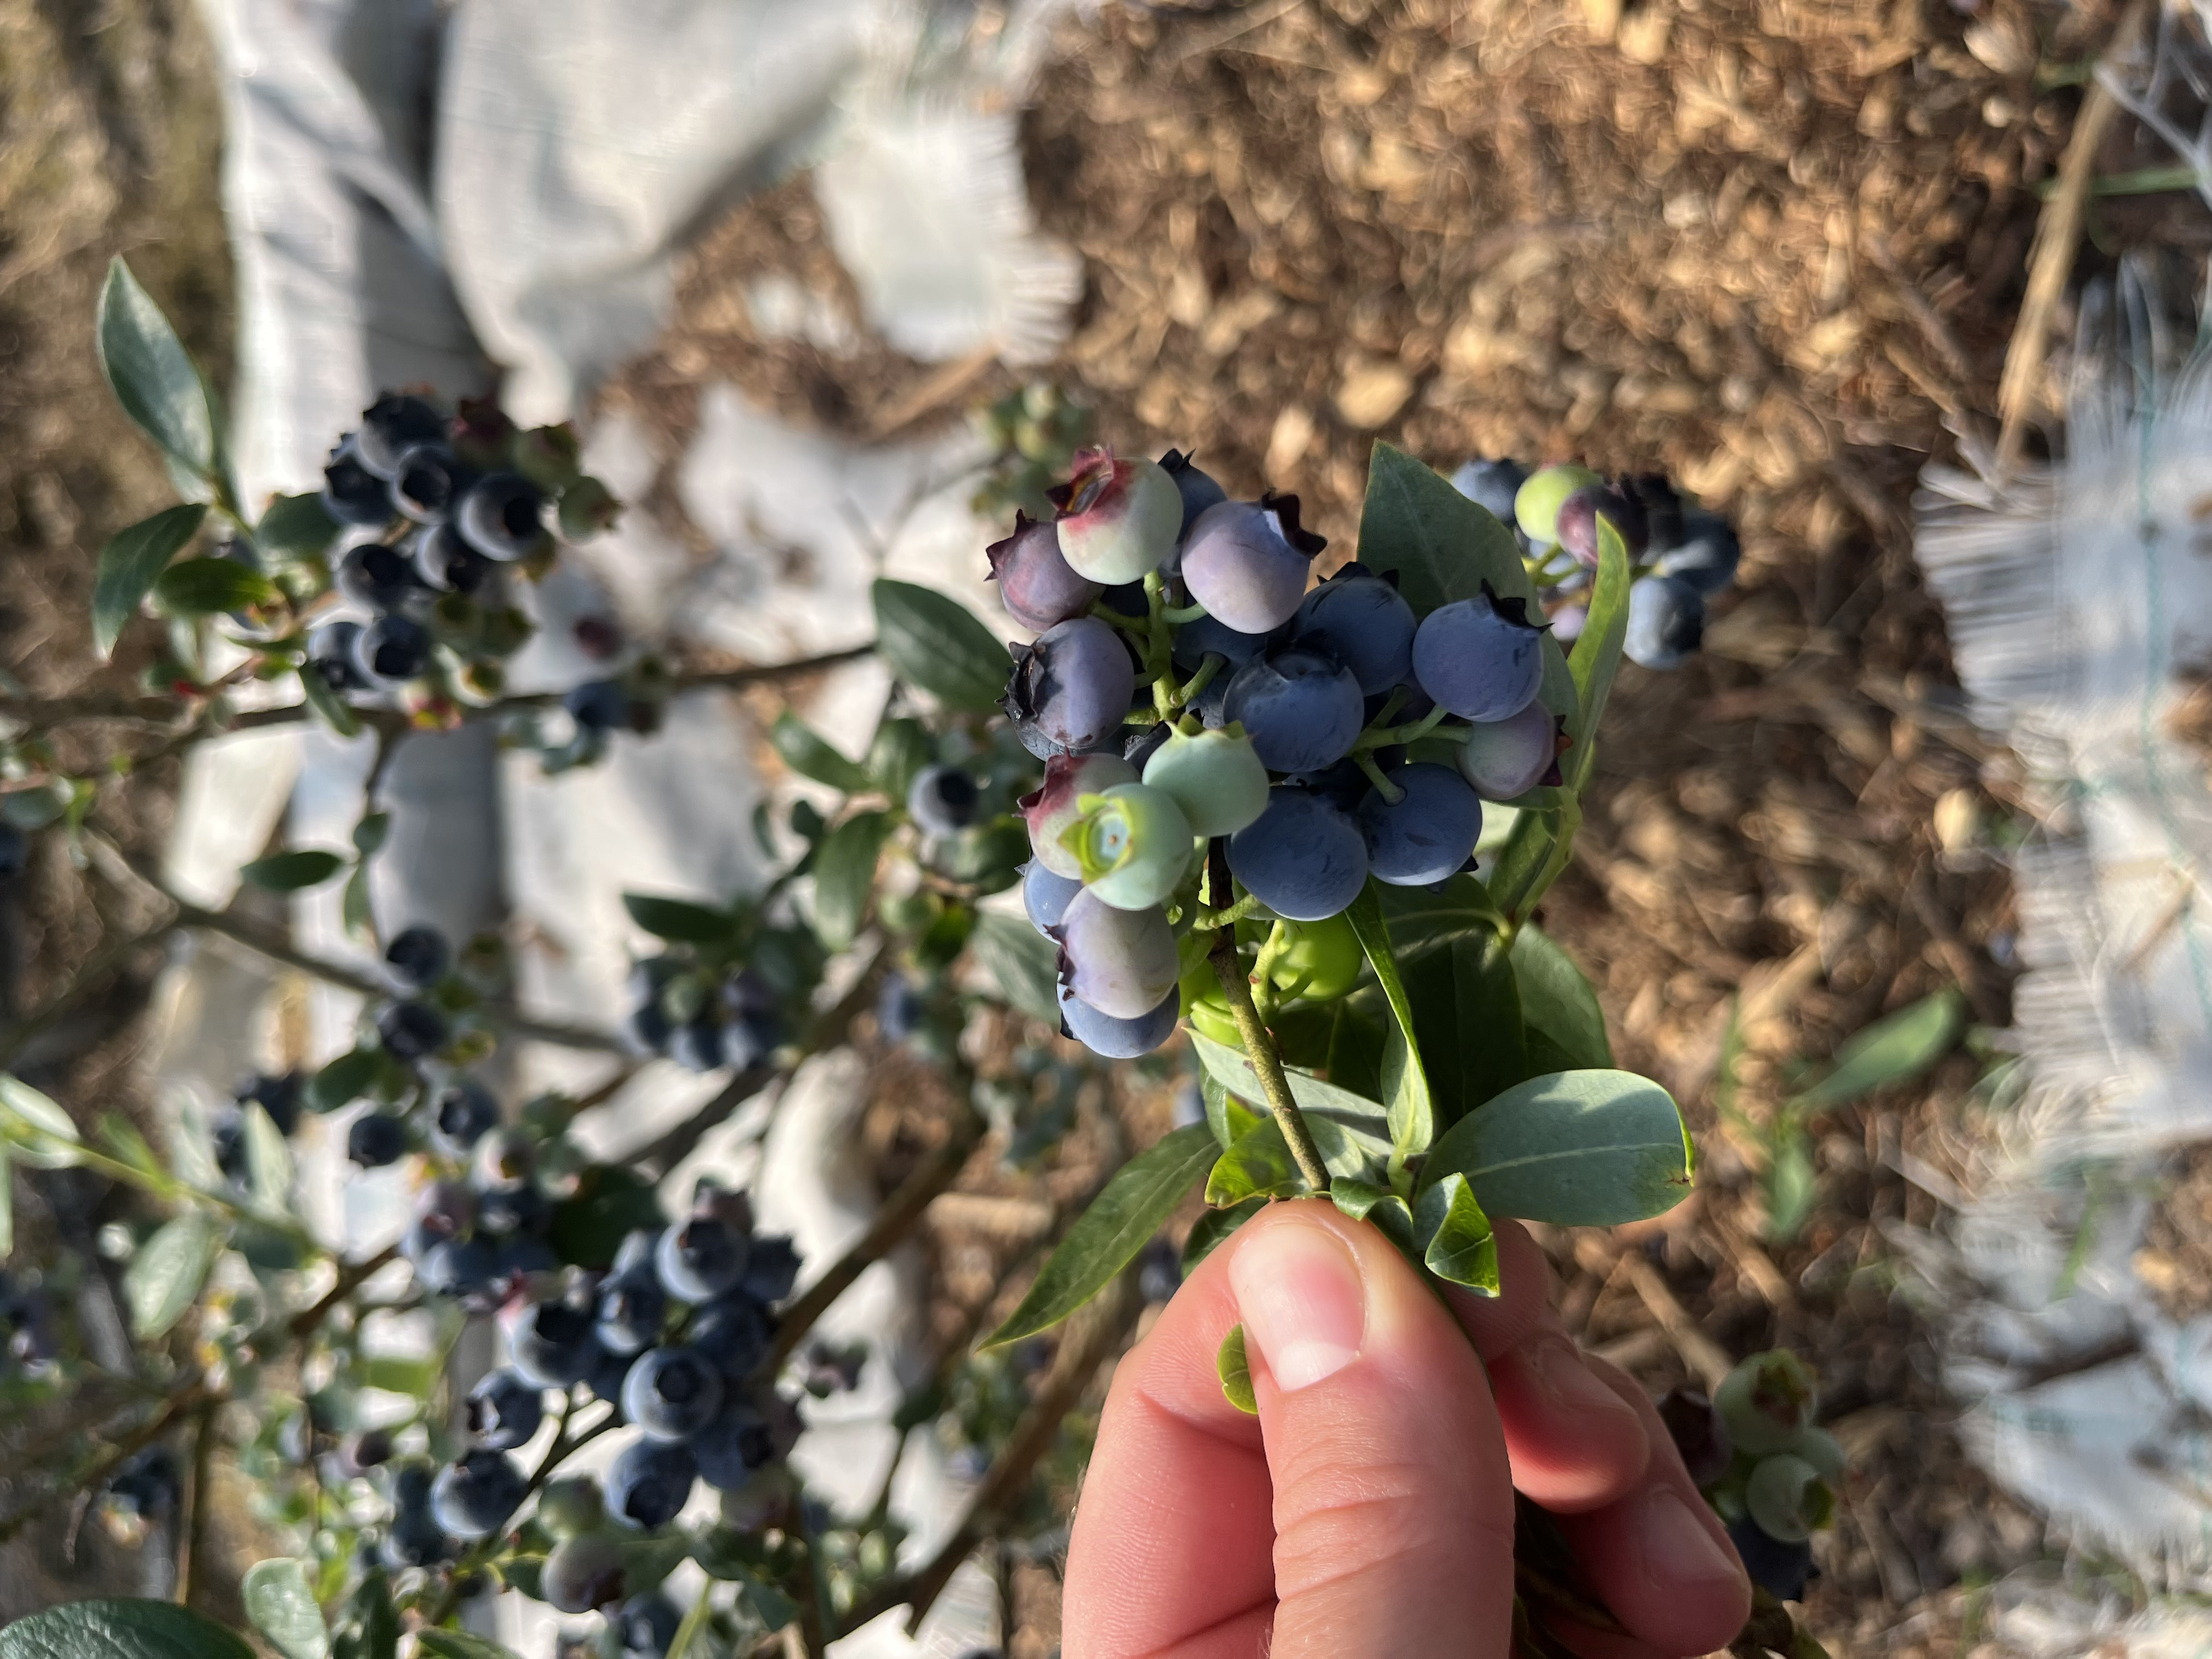
\includegraphics[width=\textwidth]{slike/borovnice.jpeg}
  \end{columns}
\end{frame}
 
% 4. Raziskovalno vprašanje in cilj
\begin{frame}{Cilj naloge}
  \begin{block}{Raziskovalno vprašanje}
    Katera metoda in kateri model sta najprimernejša za zaznavanje in razmejevanje posameznih borovnic in zakaj?
  \end{block}
  \begin{itemize}
    \item Teoretični del: učenje modelov, konvolucijske nevronske mreže, metode za zazavanje in razmejevanje posameznih objektov ter vrednotenje
    \item Aplikativni del: primerjava modelov na množici slik borovnic
  \end{itemize}
\end{frame}

 
% 5. Pregled področja in glavni rezultati
\begin{frame}{Pregled področja in glavni rezultati}
  \begin{itemize}
    \item Najpogosteje uporabljen YOLO (zadnja različica YOLO26) za zaznavanje in razmejevanje
    \item SAM2 (Segment Anything Model) za razmejeanje posameznih objektov
    \item Nadgrajen YOLO11n-seg, uporabljen na borovnicah (2025)
    \item GeCo2 za zaznavanje
  \end{itemize}
\end{frame}

% 11. Evaluacija
\begin{frame}{Vrednotenje modelov}
  \begin{block}{Definicija}
    Postopek ocenjevanja uspešnosti modela na podlagi izbranih metrik, s katerim ugotavljamo točnost njegovih napovedi, analiziramo napake in preverjamo sposobnost posploševanja na podatke, ki jih model med učenjem še ni videl.
  \end{block}
  \begin{columns}[T]
    \column{0.48\textwidth}
    \textbf{Zaznavanje}
    \begin{itemize}
      \item mAP@0.5, mAP@0.5:0.95
      \item preciznost(precision), priklic (recall), mera F1
    \end{itemize}
    \column{0.48\textwidth}
    \textbf{Razmejevanje posameznih objektov}
    \begin{itemize}
      \item IoU, Dice
      \item mask mAP
    \end{itemize}
  \end{columns}
  \vspace{0.5em}
\end{frame}
 
% 12. Načrt dela
\begin{frame}{Načrt dela}
  \begin{enumerate}
    \item Teoretični del (zaznavanje, razmejevanje posameznih objektov)
    \item Označevanje posnetih slik
    \item Učenje modelov
    \item Vrednotenje in primerjava modelov
  \end{enumerate}
\end{frame}

% LITERATURA:
% https://www.mdpi.com/2077-0472/15/15/1697
% Simon J. D. Prince (2023): Understanding Deep Learning
\end{document}